\begin{figure}[t!]
  \centering
  \begin{subfigure}{\columnwidth}
    \centering
    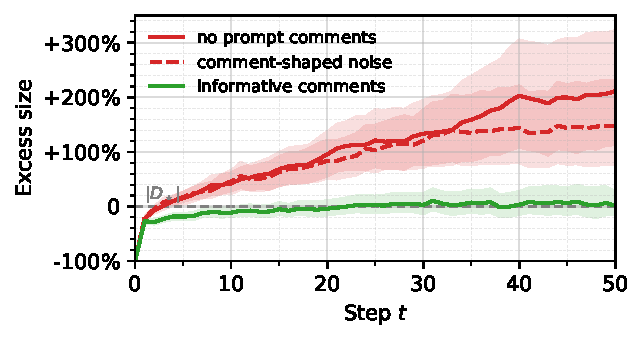
\includegraphics[width=\columnwidth]{assets/fig_causal.pdf}
    \caption{
      \textbf{Causal:} Prompts without comments (or with comment-shaped noise) grow without bound; with
      informative comments, they settle near the optimal size at equal correctness. Excess size is
      $\frac{\lvert D_t \rvert}{\lvert D_\star \rvert}{-}1$ for optimal IFEval prompt $D_\star$;
      bands are 95\% bootstrap over \HorizonWorlds{} worlds.
    }
    \label{fig:hero:lab}
  \end{subfigure}
  \begin{subfigure}{\columnwidth}
    \centering
    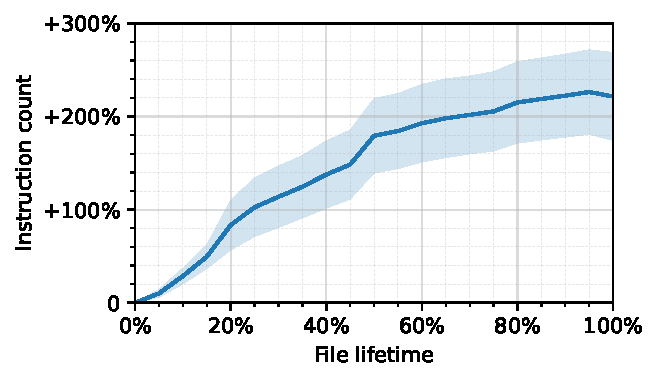
\includegraphics[width=\columnwidth]{assets/fig_growth.pdf}
    \caption{
      \textbf{Observational:} After creation, the number of prompt instructions in an agentic README
      more than triples (\FieldGrowthCountPeakPct{}) over the file's lifespan, across \FieldRepos{} GitHub
      repositories and \FieldSpells{} instruction lifetimes. Instruction count relative to file's first
      version, $\frac{\lvert D_t \rvert}{\lvert D_0 \rvert}{-}1$; lifetime normalized per file.
    }
    \label{fig:hero:growth}
  \end{subfigure}
  \caption{
    Deleting prompt instructions requires remembering why they were added; agentic prompts lack comments, so
    they only grow over their lifetime.
  }
  \label{fig:hero}
\end{figure}
